\documentclass{article}
\usepackage{t1enc}
\usepackage[magyar]{babel}
\usepackage[utf8]{inputenc}
\usepackage{times}
\usepackage{fullpage}
\usepackage{enumitem}
\usepackage{graphicx}
\title{Számítógép-architektúrák -- kidolgozott tételsor}
\author{Balázs Botond}
\begin{document}
\maketitle

\section{előadás}

\subsection{Digitális számítógép. Strukturált számítógép-felépítés. Nyelvek, szintek, virtuális gépek. Korszerű többszintű számítógépek.}

\subsubsection{Digitális számítógép}

A \emph{digitális számítógép} problémákat old meg a neki adott utasítások végrehajtása által. A \textit{program} olyan utasítássorozat, mely megadja az adott problémát megoldó algoritmust.A számítógép digitális áramkörei egyszerű utasítások korlátozott halmazát ismerik fel és hajtják végre. Minden programot ilyen utasításokká kell konvertálni végrehajtás előtt.

\textit{Gépi nyelv:} az ilyen utasítások összessége, ennek segítségével kommunikálhatunk a számítógéppel.

\begin{itemize}
	\item Elemi utasításokból áll
	\item Elektronikus áramkörökkel valósítják meg
	\item Kompromisszum az ár és a bonyolultság között
	\item A felhasználók számára nehézkes, bonyolult használat
\end{itemize}

\subsubsection{Strukturált számítógép-felépítés; nyelvek, szintek, virtuális gépek}

A bonyolultságot egymásra épülő absztrakciós szintekkel próbáljuk kezelni. Nevezzük a számítógép áramkörei által értelmezett gépi nyelvet $L_0$-nak, és vegyünk egy magasabb szintű, a felhasználó számára kényelmesebb $L_1$ nyelvet. Az $L_1$ nyelven írt programok végrehajtására ekkor két stratégiát használhatunk:

\begin{enumerate}
	\item \textbf{Fordítás}
		\begin{itemize}
			\item A \emph{fordító} végzi
			\item $L_1$ nyelvű program minden utasítását ekvivalens $L_0$ utasításokkal helyettesítjük
			\item A létrejött, tisztán $L_0$ nyelvű programot hajtja végre a számítógép, $L_1$-et eldobjuk			
		\end{itemize}
	\item \textbf{Értelmezés}
		\begin{itemize}
			\item Az \emph{értelmező} végzi
			\item A számítógépet az $L_0$ nyelven megírt értelmező vezérli az $L_1$ nyelvű program alapján
			\item Az értelmező bemenete az $L_1$ nyelvű program, minden utasítást elemez, majd azonnal végrehajt
		\end{itemize}
\end{enumerate}

Nevezzük a valódi, $L_0$ nyelvet értelmezni képes számítógépet $M_0$-nak. Az $L_1$ nyelv pedig egy $M_1$ \emph{virtuális gép} nyelvének tekinthető. Elképzelhető az $M_1$-re és az $L_1$ re épülő $M_2$ virtuális gép és $L_2$ nyelv is. Az ilyen, egymásra épülő absztrakciókat alkalmazó módszert hívjuk \emph{strukturált számítógép-felépítésnek}. Fontos megjegyezni, hogy bármely virtuális gép is megépíthető lenne fizikailag, de nagyon drága és bonyolult lenne.

$$M_0(L_0) \leftarrow M_1(L_1) \leftarrow M_2(L_2) \leftarrow ... \leftarrow M_n(L_n)$$

\subsubsection{Korszerű többszintű számítógépek}
\paragraph{-1. Eszközszint}
	A számítógép áramkörei; elektronikai tervezés eredménye.

\paragraph{0. Digitális logika}
\begin{itemize}
	\item Analóg alkaltrészekből (pl. tranzisztor) álló logikai kapuk
	\item Egy vagy több bemeneten 0 vagy 1 értéket kap
	\item Kimenete egyszerű logikai függvények eredménye (ÉS, VAGY, stb.)
	\item Egybites memória állítható össze belőlük
\end{itemize}

\paragraph{1. Mikroarchitektúra}
\begin{itemize}
	\item ALU (Aritmetikai-logikai egység): 8-32 elemű regiszterkészlete van, egyszerű matematikai műveleteket valósít meg
	\item Adatút: regiszter kiválasztása $\rightarrow$ művelet elvégzése $\rightarrow$ eredmény tárolása
	\item Mikroprogram vezérli, közvetlenül a hardver hajtja végre a műveleteket
\end{itemize}

\paragraph{2. Utasításrendszer-architektúra (ISA, Instruction Set Architecture)}
\begin{itemize}
	\item Az utasításkészlet processzorgyártó által kiadott referenciakönyve definiálja
	\item Mikroprogram interpretálja, vagy közvetlenül a hardver hajtja végre
\end{itemize}

\paragraph{3. Operációs rendszer gépi szintje}
\begin{itemize}
	\item A legtöbb ISA-utasítás megmarad (párat esetleg letilt)
	\item Új, interpretált utasítások
	\item Más memóriaszervezés
	\item Esetleg többfeladatosság, többfelhasználós működés
\end{itemize}

\paragraph{4. Assembly nyelv}
\begin{itemize}
	\item Az 1-3 szintek nyelveinek olvasható formája (általában a 3.)
	\item Fordítás a célszintre, majd interpretálás az adott szinten
\end{itemize}

\paragraph{5. Problémaorientált nyelv}
\begin{itemize}
	\item Magas szintű nyelvek (C, C++, Java, Python, stb.)
	\item \textbf{Fordítóprogram} a 3. vagy 4. szintre fordítja, majd az eredmény értelmeződik, vagy
	\item \textbf{Értelmező} hajtja végre
\end{itemize}

Egy szint \textbf{architektúráját} az általa biztosított \emph{adattípusok}, \emph{műveletek}, \emph{szolgáltatások} határozzák meg. Előbbiek az adott szint felhasználója által látható dolgok (interfész). Az ilyen interfészek tervezése a \emph{számítógép-architektúra}, bár a kifejezést számítógépek építésére is használják.

\subsection{A többszintű számítógépek fejlődése. A mikroprogramozás feltalálása. Az operációs rendszer feltalálása. Szolgáltatások átterelése a mikroprogram szintjére. Mikroprogramok száműzése.}

\subsubsection{Többszintű számítógépek fejlődése}

A \emph{hardver} a számítógép áramköreit, memóriáját és bemeneti/kimeneti (B/K, I/O) eszközeit jelenti. A \emph{szoftver} az algoritmusok számítógépes leképezése (program). A hardver és a szoftver \emph{logikailag ekvivalens}: bármilyen szoftver elméletileg megépíthető hardveresen, és bármilyen hardver emulálható szoftveresen.

\subsubsection{A mikroprogramozás feltalálása}

Az 1940-es évek számítógépei kétszintűek (ISA, digitális logika) voltak. Az ilyen gépek bonyolultak, nehezen érthetők és megépíthetők, áramköreik megbízhatatlanok.

1951-ben \emph{Maurice Wilkes} háromszintű architektúrát javasol, ez drasztikusan leegyszerűsíti és megbízhatóbbá teszi a hardvert. Az ISA-szintű programot egy beépített értelmező, a \emph{mikroprogram} hajtja végre. A hardver által támogatott utasításkészlet így jelentősen lecsökkenhet.

Az 1970-es évekre a mikroprogramozás elve uralkodóvá vált.

\subsubsection{Az operációs rendszer feltalálása}

A számítógépeket eleinte maguk a programozók kezelték -- ők készítették és töltötték be a lyukkártyákat, stb. Ez gyakori várakozáshoz és álláshoz vezetett.

1960-ban a gépkezelési feladatok automatizálására létrejött az első \emph{operációs rendszer}, az FMS (Fortran Monitor System). Ez három kezdetleges rendszerhívást (\texttt{*JOB}, \texttt{*FORTRAN}, \texttt{*DATA}) tartalmazott, mely az operációs rendszer gépi szintje kezdeményének tekinthető. Később az úgynevezett \emph{kötegelt rendszerek} bemenetüket lyukkártyáról olvasták, kimenetüket sornyomtatóra írták. Az \emph{időosztásos} rendszerek többfeladatos, többfelhasználós rendszerek voltak, melyeket távoli terminálokról, telefonon keresztül is el lehetett érni.

\subsubsection{Szolgáltatások átterelése a mikroprogram szintjére}

A mikroprogram bővítésével új, kényelmes, de redundáns utasítások jöttek létre. Ilyen volt pl. az \texttt{INC}, amely az \texttt{ADD} speciális esete, ahol az egyik argumentum 1. Ezek kicsit gyorsabbak voltak, mint az általános utasítások.

Példák komplex utasításokra:

\begin{itemize}
	\item Egészosztás
	\item Szorzás
	\item Lebegőpontos aritmetika
	\item Eljáráshívás
	\item Tömbkezelés
	\item Program mozgatása memórián belül
	\item Megszakítások
	\item Program felfüggesztése, másik folytatása
	\item Multimédiás fájlok feldolgozása
\end{itemize}

\subsubsection{A mikroprogramok száműzése}

A mikroprogramok a komplex utasítások elburjánzása miatt nagyok, lassúak lettek. Az utasításkészlet drasztikus csökkentésével és a megmaradó utasítások közvetlen végrehajtásával jelentős teljesítményjavulást lehetett elérni.

\section{előadás}

\subsection{A Neumann-elvű gép főbb részei. Központi memória: felépítése, felosztása, mérete.}

\subsubsection{A Neumann-elvű gép főbb részei}

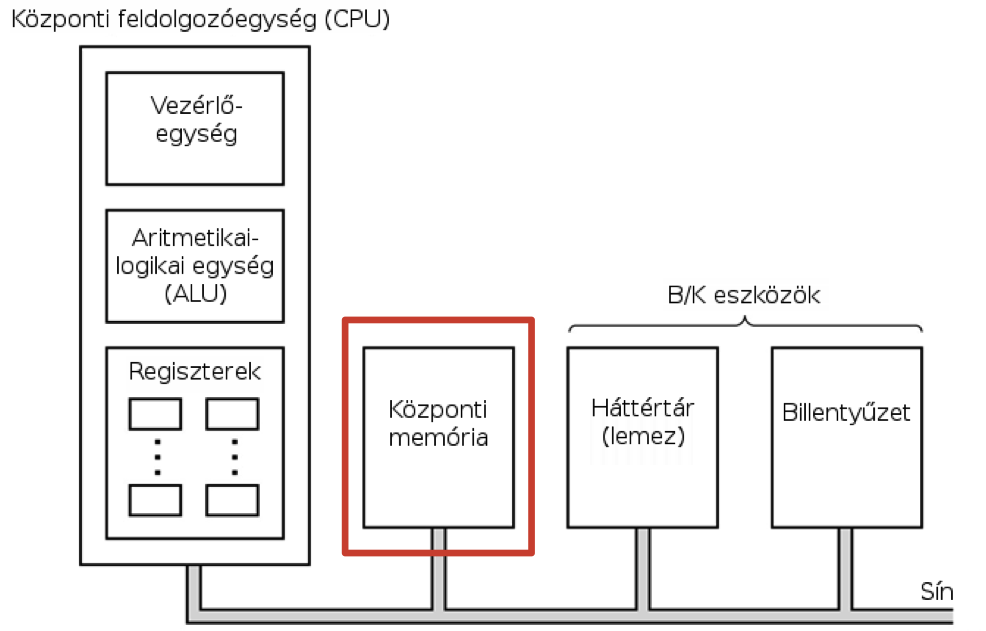
\includegraphics[width=\textwidth]{neumann}

A \emph{központi memória} a program kódját és adatait tartalmazza számokként tárolva. A \emph{központi feldolgozóegység} a központi memóriában tárolt program utasításait olvassa be és hajtja végre. A \emph{külső sín} a számítógép részegységeit köti össze; adatokat, címeket és vezérlőjeleket továbbít. A \emph{belső sín} a CPU részei közötti kommunikációt teszi lehetővé. A \emph{bemeneti-kimeneti eszközök} segítségével valósul meg a kapcsolat a felhasználóval és az adattárolás (háttértárolón).

Ezen kívül egyéb, a \emph{működést segítő eszközök} tartoznak a számítógéphez, mint például a gépház és a tápegység.

\subsubsection{Központi memória}

\paragraph{Felépítése} A tárolás alapegysége a \emph{bit}, mely 0 vagy 1 értéket vehet fel. Ezt elektronikusan az áram jelenlétével vagy hiányával ábrázolják. Legkisebb címezhető egysége a \emph{rekesz (cella)}, mely egymást követő biteket tartalmaz. Egy rekesz leggyakrabban 8 bites (\emph{bájt}), de korábban ettől eltérő csoportosítással is lehetett találkozni.

A memóriarekeszek tartalmát címük alapján érhetjük el. Egyes gépeken a memóriát egydimenziós tömbnek tekinthetjük, melynek indexei a memóriacímek. Máshol a kis címhossz miatt szegmensekre osztják a memóriát, és a szegmens és egy ennek kezdőpontjához képesti eltolás megadásával címezhetünk meg egy rekeszt (\emph{szegmens:offszet címzés}). Ezeken kívül számos egyéb címzési mód létezik.

A számítógép egy regiszterébe beférő bájtokat \emph{szónak} nevezzük. A szó tehát 32-bites rendszeren 4, 64-bitesen 8 bájtot jelent. Sok gépi kódú utasítás teljes szavakkal dolgozik.A memóriában általában tetszőleges bájtot megcímezhetünk, de a szóhatáron kezdődő címek elérése gyorsabb. A fordítóprogramok általában képesek szóhatárra igazítani az adatokat.

A rekeszek adatokat (pl. egész, lebegőpontos, BCD szám, karakterkód, stb.) vagy gépi kódot tartalmazhatnak. A gépi kódú utasítások és ezek operandusai is számok.

\paragraph{Felosztása} A memória nagy részét a programok szabadon használhatják, bizonyos címterületek azonban a hardverrel való kapcsolattartásra vannak fenntartva. Bizonyos címek meghatározhatják egyes címterületek tartalmát (pl. RAM vagy ROM legyen ott elérhető).

\paragraph{Mérete} Korábban pár kilobájtos, megabájtos volt, ma több gigabájt az általános.

\subsection{Utasítás-végrehajtás. Utasítás- és processzorszintű párhuzamosság. RISC és CISC. Korszerű számítógépek tervezési elvei.}

% A \emph{CPU} (Central Processing Unit, Központi Feldolgozóegység) feladata a központi memóriában tárolt programok végrehajtása. Ez az utasítások beolvasását, vizsgálatát, majd egyenkénti elvégzését jelenti.

% A számítógép komponenseit \emph{sín} (bus) köti össze, ez cím-, adat- és vezérlőjeleket továbbító párhuzamos vezetékek kötege.

% A CPU több önálló részegységből áll. A \emph{vezérlőegység} (Control Unit, CU) beolvassa az utasításokat a központi memóriából, és eldönti, hogy milyen típusúak. Az \emph{aritmetikai-logikai egység} (Arithmetic Logic Unit, ALU) az utasítások végrehajtásához szükséges matematikai és logikai műveleteket végzi el.

% A CPU-ban kis méretű, nagy sebességű memóriarekeszek, regiszterek is vannak, midegyiknek meghatározott mérete és funkciója van. Általában minden regiszter azonos méretű. A legfontosabb regiszter a \emph{programszámláló} (Program Counter, PC), amely a következő végrehajtandó utasítás memóriacímét tartalmazza. Az \emph{utasításregiszterben} (Instruction Register, IR) pedig az épp végrehajtott utasítást találjuk.

\end{document}